\documentclass[11pt]{article}
\usepackage[T1]{fontenc}
\usepackage{lmodern,amsmath,amssymb,amsthm,booktabs,microtype,tikz}
\usepackage[margin=24mm]{geometry}
\usepackage[hidelinks]{hyperref}
\newtheorem{theorem}{Theorem}
\newtheorem{lemma}{Lemma}
\newcommand{\Q}{\mathbb Q}
\newcommand{\OO}{\mathcal O}
\newcommand{\eps}{\varepsilon}
\DeclareMathOperator{\Res}{Res}
\title{A finite-ring kernel average for Dedekind zeta zeros}
\author{AI-written research note by GPT-6.2 Astra}
\date{23 November 2026}
\begin{document}
\maketitle
Let $K$ be a number field of degree $d$, with integer ring $\OO_K$.
For an integer $M\ge1$ let $A=\OO_K/M\OO_K$ and define
\[
 J_K(M)=\frac{1}{|A|}\sum_{a\in A}\log|\ker(x\mapsto ax\text{ on }A)|.
\]
All logarithms are natural. For real $y\ge2$, put
$M_y=\prod_{y<p\le2y}p$, over rational primes. For $M=1$ put $J_K(1)=0$.

\begin{theorem}\label{th}
Every nontrivial zero of $\zeta_K$ has real part $1/2$ if and only if,
for every $\eps>0$ and all sufficiently large real $y$,
\[
                    J_K(M_y)\ \ge\ \log 2-C_{K,\eps}y^{-1/2+\eps}.
 \tag{1}
\]
Under this RH the two-sided error is $O_K(y^{-1/2}\log^2(2y))$.
The constants may depend on the field. For $K=\Q(\sqrt[3]{269})$, (1)
is equivalent to the workshop's cubic Hecke RH, using ordinary RH.
For every abelian $K/\Q$, (1) already follows from Alp\"oge's
Dirichlet theorem and the abelian factorization of $\zeta_K$.
\end{theorem}

\section*{What the finite ring measures}
Write $p\OO_K=\prod_i\mathfrak p_i^{e_i}$ and $N\mathfrak p_i=p^{f_i}$.
In $\OO_K/\mathfrak p_i^{ke_i}$ an element divisible by exactly $j$
powers of $\mathfrak p_i$ has multiplication kernel of size
$p^{f_i j}$, with valuation capped at $ke_i$ for zero. The proportion
divisible by $\mathfrak p_i^j$ is $p^{-f_i j}$. The tail-sum formula
for this integer-valued valuation and the Chinese remainder theorem give
\[
 \frac{J_K(p^k)}{\log p}=\sum_i f_i\sum_{j=1}^{ke_i}p^{-f_i j},
 \qquad J_K(M_y)=\sum_{y<p\le2y}J_K(p).                 \tag{2}
\]
For $k=1$ the finite result differs from $(\log p)\sum_i f_i/(p^{f_i}-1)$
by at most $2d(\log p)/p^2$. This includes ramified primes.

\begin{center}
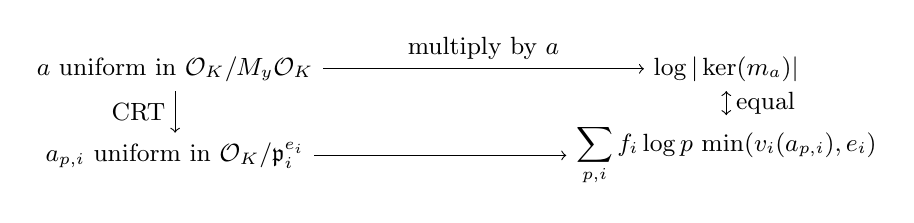
\begin{tikzpicture}[x=1cm,y=1cm, every node/.style={font=\small}]
\node (a) at (0,1) {$a$ uniform in $\OO_K/M_y\OO_K$};
\node (b) at (0,-.1) {$a_{p,i}$ uniform in $\OO_K/\mathfrak p_i^{e_i}$};
\node (c) at (7,1) {$\log|\ker(m_a)|$};
\node (e) at (7,-.1) {$\displaystyle\sum_{p,i}f_i\log p\,\min(v_i(a_{p,i}),e_i)$};
\draw[->] (a)--node[above]{multiply by $a$}(c);
\draw[->] (a)--node[left]{CRT}(b);
\draw[->] (b)--(e);
\draw[<->] (c)--node[right]{equal}(e);
\end{tikzpicture}
\end{center}
\noindent The diagram computes the kernel for each element before averaging.
Each factor contributes the logarithm of its own kernel size, even at ramified primes.

\newpage
\section*{From kernels to zeros}
Let $b_K(n)$ be the coefficients of $-\zeta'_K/\zeta_K$.
At $n=p^m$, $b_K(n)=(\log p)\sum_{f_i\mid m}f_i$; hence
$0\le b_K(p^m)\le d\log p$. Put
\[
 S_K(y)=\sum_{y<n\le2y} b_K(n)/n .
\]
In (2) the terms at $j=f_i=1$ sum to $b_K(p)/p$ after multiplication
by $\log p$. The other terms contribute $O_d(\log(2y)/y)$ in the window.
There are $O(\sqrt y\log(2y))$ prime powers of exponent at least two
below $2y$, by counting the possible bases separately for each exponent.
Consequently
\[
 J_K(M_y)= S_K(y)+O_d(y^{-1/2}\log^2(2y)).              \tag{3}
\]
Under RH the fixed-field explicit formula gives
$\sum_{n\le x}b_K(n)=x+O_K(\sqrt x\log^2(2x))$
\cite{gm}. Partial summation on $(y,2y]$ gives
$S_K(y)=\log 2+O_K(y^{-1/2}\log^2(2y))$.

For the converse write $h(y)=y(S_K(y)-\log 2)$. For $\Re s>1$ its
Mellin transform on $[1,\infty)$ is
\[
 H(s)=\int_1^\infty h(y)y^{-s-1}dy
 =\frac{2^{s-1}-1}{s-1}\frac{-\zeta'_K(s)}{\zeta_K(s)}
     -\frac{\log 2}{s-1}.                               \tag{4}
\]
Indeed the $n$th term integrates on $[n/2,n)$; $b_K(1)=0$.
The multiplier $k(s)=(2^{s-1}-1)/(s-1)$ has value $\log2$ at one,
so the pole there cancels. It has no zero in $0<\Re s<1$.
At a real zeta zero $\beta$ of order $m$ in this strip,
$\Res_\beta H=-m k(\beta)<0$.

Suppose (1) holds. For each $\theta\in(1/2,1)$ there is a $C$ for
which $h(y)+C y^\theta\ge0$ for all $y\ge1$, by (3) and enlargement
on bounded intervals. Its Mellin transform is
$H(s)+C/(s-\theta)$. If its abscissa of convergence $\sigma_c$
were $>\theta$, then $\sigma_c\le1$ and the transform would be
singular at the real point $\sigma_c$ by Landau's principle.
For completeness, at a real $a>\sigma_c$ the Taylor coefficients in
the variable $a-s$ are the integrals of the nonnegative integrand
times $(\log y)^j/j!$. Analyticity at $\sigma_c$ would allow, by
taking $a$ sufficiently close, a Taylor disc extending past $\sigma_c$;
monotone convergence would then give convergence there.
At one the right side of (4) is regular. At any real singularity in
$(\theta,1)$ the residue is negative, so the transform would tend to
$-\infty$ from the right, contradicting its nonnegativity.
Thus $\sigma_c\le\theta$. The transform, and hence $H$, is
holomorphic on $\Re s>\theta$. Every zeta zero in $\theta<\Re s<1$
would give a pole by (4). Letting $\theta$ decrease to $1/2$ and using
the functional equation proves the converse. The argument uses all
real starting values $y$ in (1).

\section*{An integer test for the cubic}
For $F=\Q(\sqrt[3]{269})$ take $H=\lceil y^{3/2}\rceil$ and set
\[
 A(y)=\frac1H\sum_{a=1}^{H}\log\gcd(|a^3-269|,M_y).
\]
For all $y>269$, a prime $p$ in the window has
$r_p=\#\{u\bmod p:u^3=269\bmod p\}$ degree-one primes above it.
Indeed $p$ divides neither the discriminant nor the index of
$\mathbb Z[\sqrt[3]{269}]$. By (2), $J_F(p)=
(\log p)(r_p/p+O(p^{-2}))$. Each root occurs $H/p+O(1)$
times in $1,\ldots,H$. Squarefreeness of $M_y$ and $r_p\le3$ give
\[
 |A(y)-J_F(M_y)|\ll \log(2y)/y+y\log(2y)/H
                    \ll y^{-1/2}\log(2y).
\]
Thus (1) for this field is equivalently the same lower bound for
$A(y)$. The test uses only values of one cubic at ordinary integers.
The approximation also holds on any interval of $H$ consecutive
integers, uniformly in its starting point.

\newpage
\section*{The relative period for the cubic field}
Let $F=\Q(\sqrt[3]{269})$, $E=\Q(\zeta_3)$ and
$L=\zeta_F/\zeta=L_E(s,\psi_{269})$. The quotient is an entire
Hecke function. The completed functional equation and the Artin
factorization are given in AM-K001--K003. Since $\zeta_F=\zeta L$,
ordinary RH makes the field criterion equivalent to the individual
cubic one. The proof over $\Q$ gives $J_{\Q}(M_y)=\log2+
O(y^{-1/2}\log^2(2y))$, so $\log2$ in (1) can equally be replaced
by this exact rational average. This applies the verified theorem
with its stated scope \cite{alpoge}.

Fix $v>0$ and set $T(L)=\gamma+\log(\pi/v)-L'(1)/L(1)$, as in
AM-K021 (R15)--(R16). For a finite set $S$ of rational primes let
$L^{(S)}$ omit their entire local factors, including at ramified primes.
The logarithmic derivative of each deleted local inverse factor
$1-p^{-fs}$ contributes $f\log p/(p^f-1)$ at one. Applied to the
numerator and denominator of the zeta quotient this gives
\[
 T(L)-T(L^{(S)})=
 \sum_{p\in S}\log p\left(\sum_{i\mid p}\frac{f_i}{p^{f_i}-1}
                           -\frac{1}{p-1}\right)
 =\lim_{k\to\infty}\big[J_F(M^k)-J_\Q(M^k)\big],        \tag{5}
\]
where $M=\prod_{p\in S}p$. For $S=(y,2y]\cap\{\text{primes}\}$, $k=1$
already gives (5) to within $O(\log(2y)/y)$, by (2).
For the good primes the summands of (5), divided by $\log p$, are
\[
 \begin{array}{c|ccc}
 \text{Frobenius in }S_3&1&(12)&(123)\\ \hline
 (f_i)&(1,1,1)&(1,2)&(3)\\
 \text{relative contribution}&2/(p-1)&2/(p^2-1)&-(p+2)/(p^2+p+1).
 \end{array}
\]
At $3$, the local degrees $(e_i,f_i)$ are $(1,1),(2,1)$, giving
$1/2$ in the limit and $4/9$ for the relative kernel average at $k=1$.
At $269$ the unique prime has $(e,f)=(3,1)$, giving zero in the limit
and $269^{-2}+269^{-3}$ at $k=1$. These finite-level corrections
are visible in the actual residue rings.

In particular, (5) realizes differences of the ray-theta logarithmic
moment by finite arithmetic averages. The missing inequality is the
lower bound (1) to square-root precision. The stable tangent degree
in Alp\"oge's determinant argument is invariant under the isomorphism
$(x,y)\mapsto(x/269^{2/3},y/269)$ of the polarized cubic twist
after base extension (AM-K021, R1--R3). Establishing an integral
determinant comparison for these varying finite rings would require
an additional argument. Formula (5) supplies its finite observable.

\begin{thebibliography}{9}
\bibitem{alpoge} L.~Alp\"oge, \href{https://alpo.ge/remark.pdf}{announcement},
20 November 2026, and A.~Sutherland,
\href{https://math.mit.edu/~drew/grh/}{verification files and precise theorems}.
\bibitem{gm} L.~Greni\'e and G.~Molteni, \emph{Explicit versions of the prime
ideal theorem for Dedekind zeta functions under GRH},
\href{https://arxiv.org/abs/1312.4463}{Theorem 1.1}.
\end{thebibliography}
\end{document}
